\documentclass[11pt]{amsart}
\usepackage{geometry}                % See geometry.pdf to learn the layout options. There are lots.
\geometry{letterpaper}                   % ... or a4paper or a5paper or ... 
%\geometry{landscape}                % Activate for for rotated page geometry
%\usepackage[parfill]{parskip}    % Activate to begin paragraphs with an empty line rather than an indent
\usepackage{graphicx}
\usepackage{amssymb}
\usepackage{epstopdf}
\usepackage{enumerate}
\DeclareGraphicsRule{.tif}{png}{.png}{`convert #1 `dirname #1`/`basename #1 .tif`.png}
\setlength{\parindent}{0in} % no paragraph indent

\usepackage{fancyhdr}
\pagestyle{fancy}
\lhead{\footnotesize \parbox{11cm}{STAT 434 Data Analysis} }
\rhead{\footnotesize \parbox{11cm}{Max Scheiber and Ruslan Zagatskiy} }

\title{STAT 434 Data Analysis - Max Scheiber and Ruslan Zagatskiy}
\date{11.25.2013}

\begin{document}
\maketitle
\section{Overview}
Our goal was to explore the relationship between the NSA scandals of 2013 and securities of related tech sector stocks. \\

\section{Raw data to polished data}
We obtained consolidated trade data from Wharton Research Data Services (WRDS) for Google (GOOG), Apple (AAPL), Microsoft (MSFT), and Facebook (FB) for the January 1st, 2013 through July 31st, 2013 timespan. These consolidated datasets contain average execution prices and total shares volume a few times each second. We chose these stocks because they were the ones identified in the NSA's leaked slide deck. \\

To make data analysis more manageable, we converted this data into hourly buckets from 9am to 3pm, inclusive. We did this by taking the average execution price over each bucket, equally weighted within the bucket. (For the final presentation, it may be better to volume-weight this mean). We also took volume sums for each bucket. \\

We then created a basket of tech stocks by taking the equal-weighted average of each bucket of all stocks considered. The reason for doing this was to enhance our signal-to-noise ratio; this basket would minimize the effects in securities pricing and volatility of, say, one company's earnings report, while confirming sector-wide trends. \\

Within this basket, we computed percent returns, which allowed us to compute a scale-independent moving volatility. We currently measure volatility from a given time bucket over the previous 30 time buckets. Given that there are seven buckets per day, we see our volatility measure cover a duration of just over four days. (For the future, we may wish to model volatility with an exponential smooth.) \\

\newpage
\section{Google analysis}
Before performing analysis on the basket of stocks, we performed some basic analysis of Google's returns. \\

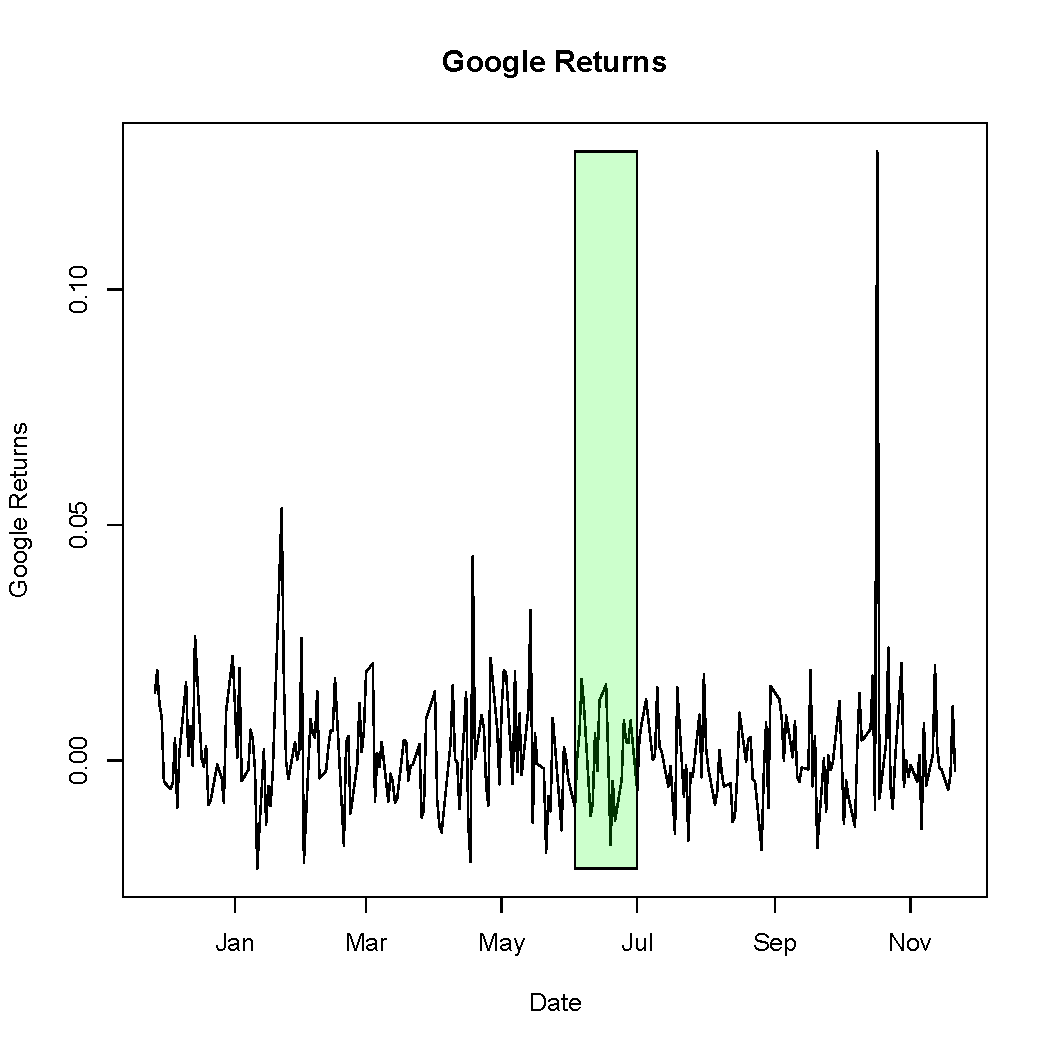
\includegraphics[scale=0.4]{goog_returns_11_25.pdf} \\

Immediately, we can see that Google did not really have any outliers in its return over the summer. Its main spikes seem to come from its earning reports, implying that the market did not judge the NSA scandals to really affect Google. \\

We next look at Google's hourly volatility throughout June, which is when the majority of the NSA leaks happened. It initially seems obvious via eyeballing that Google's volatility spiked on June 6th (the date of \textit{The Guardian}'s first leak) and June 20th (the date of \textit{The Guardian}'s second leak). \\

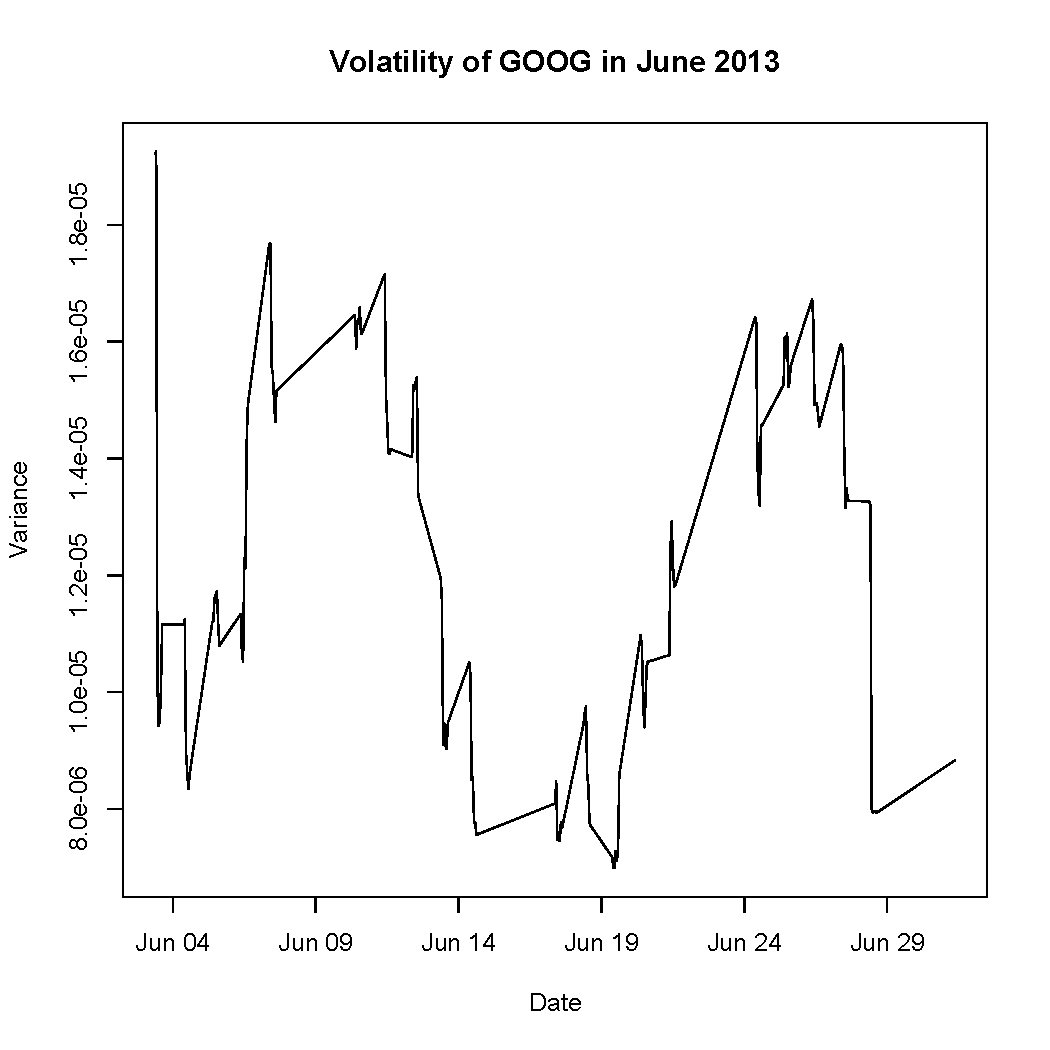
\includegraphics[scale=0.4]{goog_vol_zoom_11_25.pdf} \\

However, in context, these spikes are extremely minimal. Let us, for example, plot volatility throughout 2013. \\

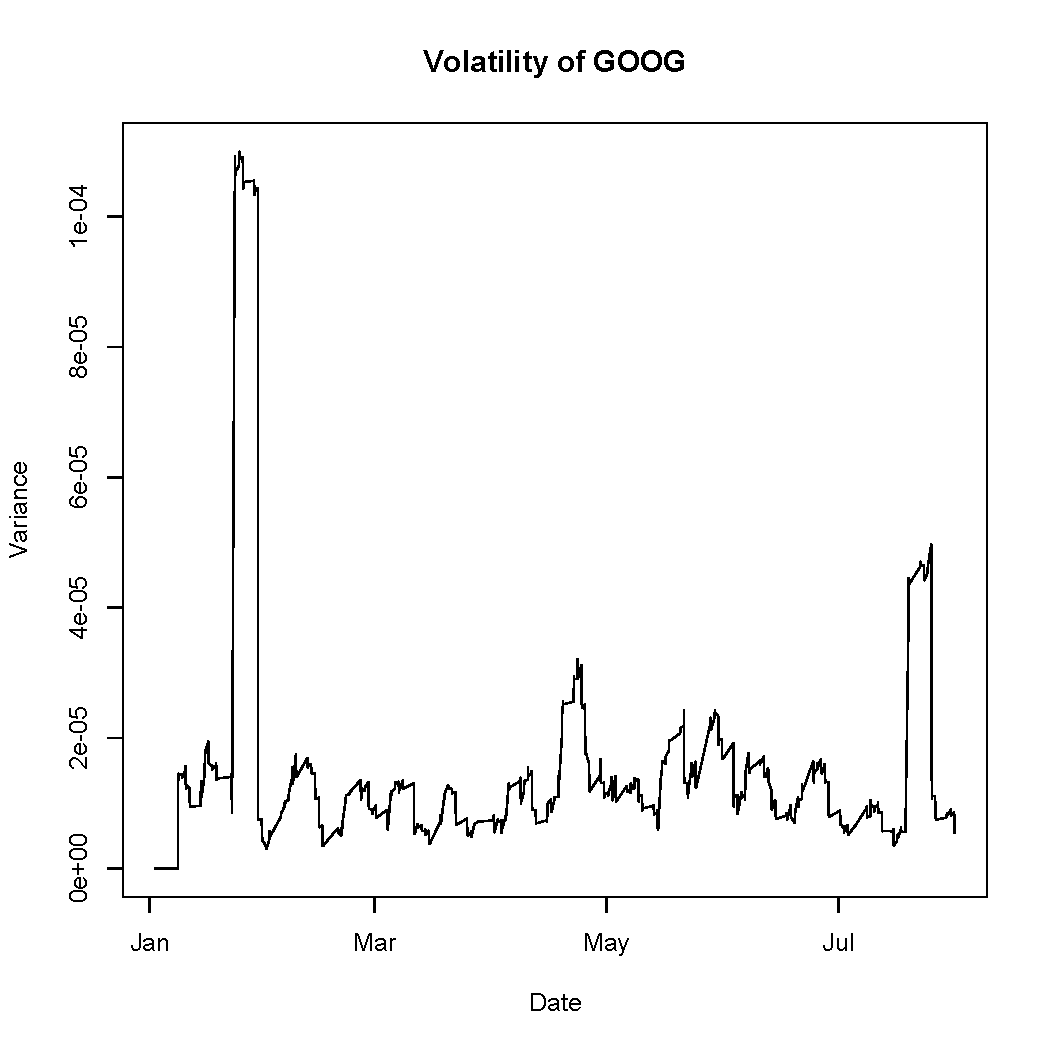
\includegraphics[scale=0.4]{goog_vol_11_25.pdf} \\

Any June spikes that could be related to the NSA do not look very significant in the context of Google's volatility throughout the year. While it is ostensible that these small June spikes may indeed have occurred as a result of the NSA scandal, this seems to be an early indicator that our hypothesis may not hold.

\newpage
\section{Tech sector basket analysis}
For further confirmation, we now look at the full tech sector basket as discussed in section 2. \\

To check for any sort of heteroskedasticity, we plot squared returns of the basket. \\

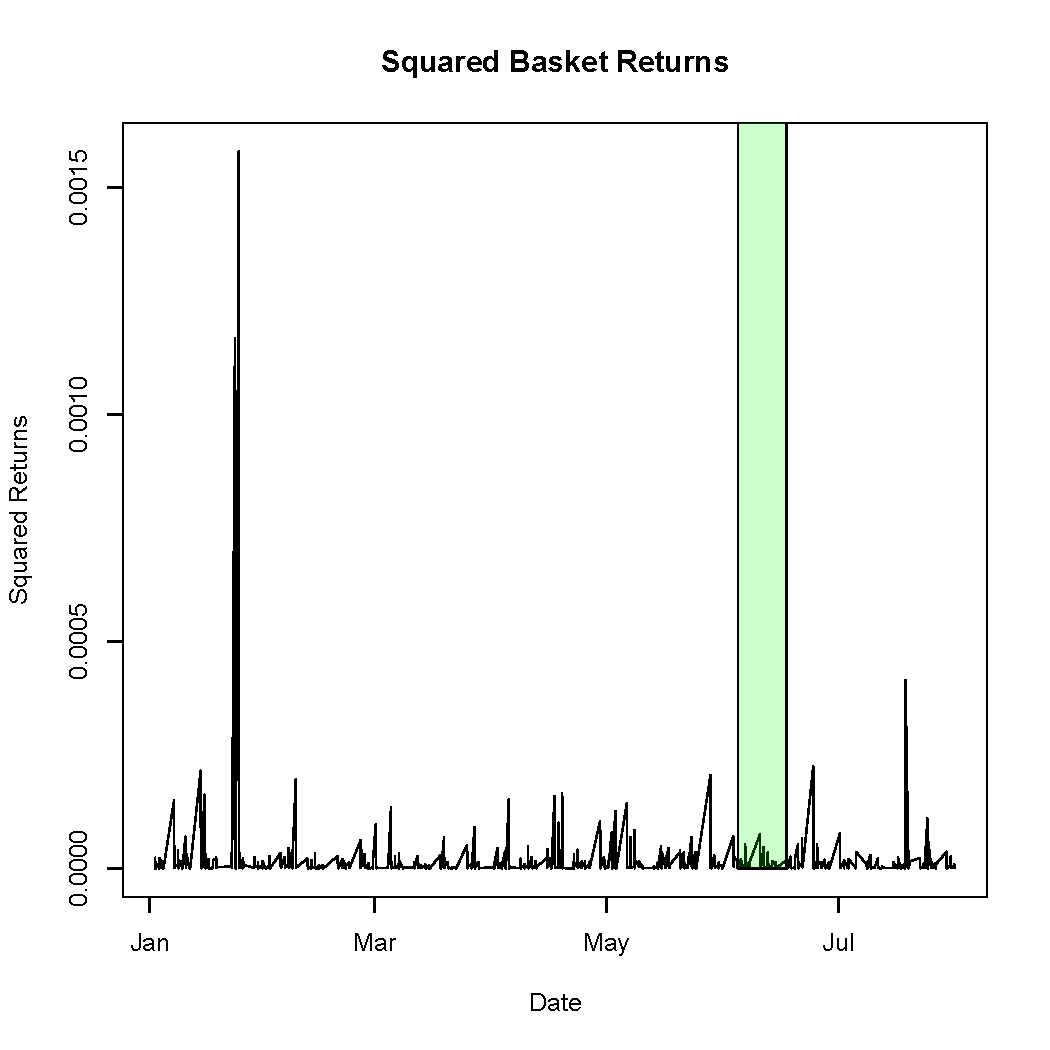
\includegraphics[scale=0.4]{basket_sq_returns_11_25.pdf} \\

\newpage
While the basket's 2013 squared returns have some unusual spikes,  it looks generally stable. More rigorously, we considered an ARCH(1) model for the basket's returns. The model's first coefficient is statistically insignificant, implying homoskedasticity. Statistically, any volatility is more or less noise. \\

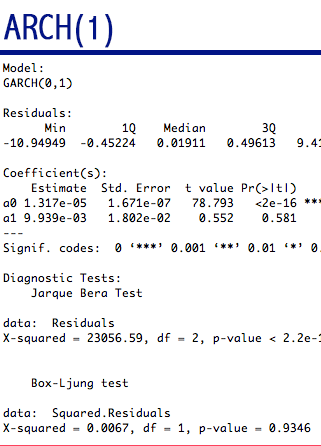
\includegraphics[scale=0.7]{arch1_basket_11_25.png} \\

\newpage
Let us try another approach - regressing on an indicator variable. We set an indicator variable to be true for all buckets on June 6th, the day of the first NSA leak, and we set another indicator variable to be true for all buckets on June 20th, the day of a large second NSA leak. We examine these indicators solely within the month of June and additionally within the entirety of 2013. We regress volatility on these indicators to test their significance. \\

The result of these regressions is that only the second NSA leak (June 20th) is statistically significant \textit{when considered within the context of June}. It is worth noting that when considered within the context of all of 2013, the June 20th leak is statistically insignificant with a  $p-value = 0.4$. The June 6th indicator does not have significant explanatory power for volatility in June or in 2013. It is arguable that \textit{The Guardian}'s leak did spur more volatility in the market, but this washes out in the long run due to other similar events that affect the tech sector. \\

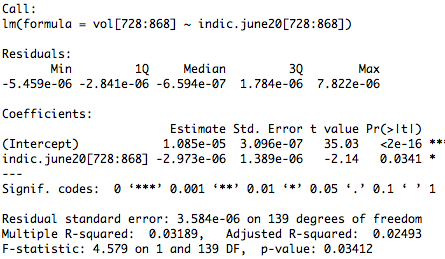
\includegraphics[scale=0.6]{june_20_june_11_25.png} \\

\newpage
\section{To come}
This data may tell us a story about the NSA scandal. Did people not realize its magnitude initially, and it took until further leaks for the market to reflect it? We would like to investigate this qualitatively through news articles and commentaries in an attempt to find particularly prominent stories. \\

We would also like to look beyond volatility with this basket of stocks, perhaps exploring trading volume per bucket. \\

In addition, we would like to consider different time horizons throughout 2013. In particular, we're interested in exploring whether the leaks changed short-term volatility in the months of July and August. \\

We would like to consider modeling our volatility using the news impact curve discussed in our research, which is a GARCH model that considers how shocks affect conditional volatility. We would also like to consider modeling volatility with an exponential smooth. \\

We expect to be finished with our analysis by the end of Thanksgiving break, hopefully coming to an interesting conclusion about the short-term impact of Snowden's leaks on the volatility of our basket. If we can find evidence for this, it might be worth considering tech stocks outside of our current basket. \\

\end{document}  